%\chapter{Research Trajectories}
%\label{future_research}
%Although we established its many benefits, DFiant is still missing a few milestones before it becomes a worthy HDL candidate. In the scope of this research, we plan to explore the following trajectories, in an effort to close this gap. We believe DFiant can be an invaluable tool for computer architecture research. 

\chapter{Research Trajectory: Advanced Dataflow Control}
\label{trajectory_dataflow}
So far, we demonstrated how DFiant can cover static one-to-one token transfer functions. Notwithstanding, functionality may require upsampling (e.g., duplicate each token), downsampling (e.g., drop every third token), token arrival time dependency (e.g., priority round-robin arbiter), or token value dependency (e.g., filter out odd-valued tokens). In this trajectory, we propose constructs and semantics to formulate such functions in DFiant.

\section{Static Dataflow Scheduling}
Static dataflow scheduling occurs when both input and output token rates are static and known at compile-time. Such scheduling manipulation can be supported by defining the following constructs:
\begin{itemize}
  \item \code{.next(step)} and \code{.assignNext(step)}\quad These enable referencing a future dataflow token value, potentially breaking \textit{Causality}. However, we naturally do not allow \code{x := x.next}, and protect these constructs, while internally utilizing them to create powerful public methods such as \code{Reusable}. We expect to translate all \code{next} references to state-machines using \code{prev}, during early compilation phases.
  \item \code{.split(num)}\quad Converts one dataflow variable into a sequence of dataflow elements, thereby creating a round-robin distribution between the elements. \code{num} determines the sequence size. Therefore, for a given $r$ token rate input, each output element receives a downsampled $r/num$ token rate. 
  \item \code{.merge(seq)}\quad Acts as the opposite of \code{split}. Converts a dataflow variable sequence into a single dataflow variable. Therefore, for a given $r$ token rate at each sequence element, the upsampled output token rate is $r*seq.length$. 
  \item \code{Reusable[Component]}\quad This construct enables utilizing the same component more than once, by creating an implicit state machine that schedules the tokens. Consider the example in Fig. \ref{fig:Reusable}, which has three possible implementations of a function that takes three dataflow arguments and outputs their sum. \code{sumA} invokes two \code{+} operations, thereby constructing two adders. \code{sumB} constructs two sequences on the adder's inputs and calls \code{merge}, thereby utilizing the same adder. \code{sumC} exposes how effective \code{Reusable} truly is. Not only that lines of code count is reduced, but the code is much simpler and the designer does not need to prepare ahead, according to the number of reuses adder incurs. Obviously, using a single adder instead of two reduces the output token rate by half.
  
  \begin{figure}[h]
    \centering
    \begin{minipage}{0.82\linewidth}
      \begin{minted}[autogobble,tabsize=2,framesep=1pt, frame=single,fontsize=\scriptsize]{scala}
        def sumA(a : DFUInt[32], b : DFUInt[32], c : DFUInt[32]) : DFUInt[32] = {
          a + b + c //sum using two adders
        }
        def sumB(a : DFUInt[32], b : DFUInt[32], c : DFUInt[32]) : DFUInt[32] = {
          val adder = DFUInt[32]
          val lhs = Seq(a, c)     //adder left-hand side
          val rhs = Seq(b, adder) //adder right-hand side
          adder := lhs.merge + rhs.merge //sum using a single adder
          adder
        }
        def sumC(a : DFUInt[32], b : DFUInt[32], c : DFUInt[32]) : DFUInt[32] = {
          val adder = Reusable[DFAdder[32, 32]] //Reusable adder of 32 bits vectors
          adder(adder(a, b), c) //sum using a single adder
        }
      \end{minted}
    \end{minipage}
    \captionof{figure}{\code{Reusable} construct example}
    \label{fig:Reusable}
  \end{figure}
\end{itemize}

\fig{fig:Dataflow} illustrates token flow through dataflow variables and how it influenced by \code{prev}, \code{next}, \code{split}, and \code{merge}.

\begin{figure}[t]
  \centering
  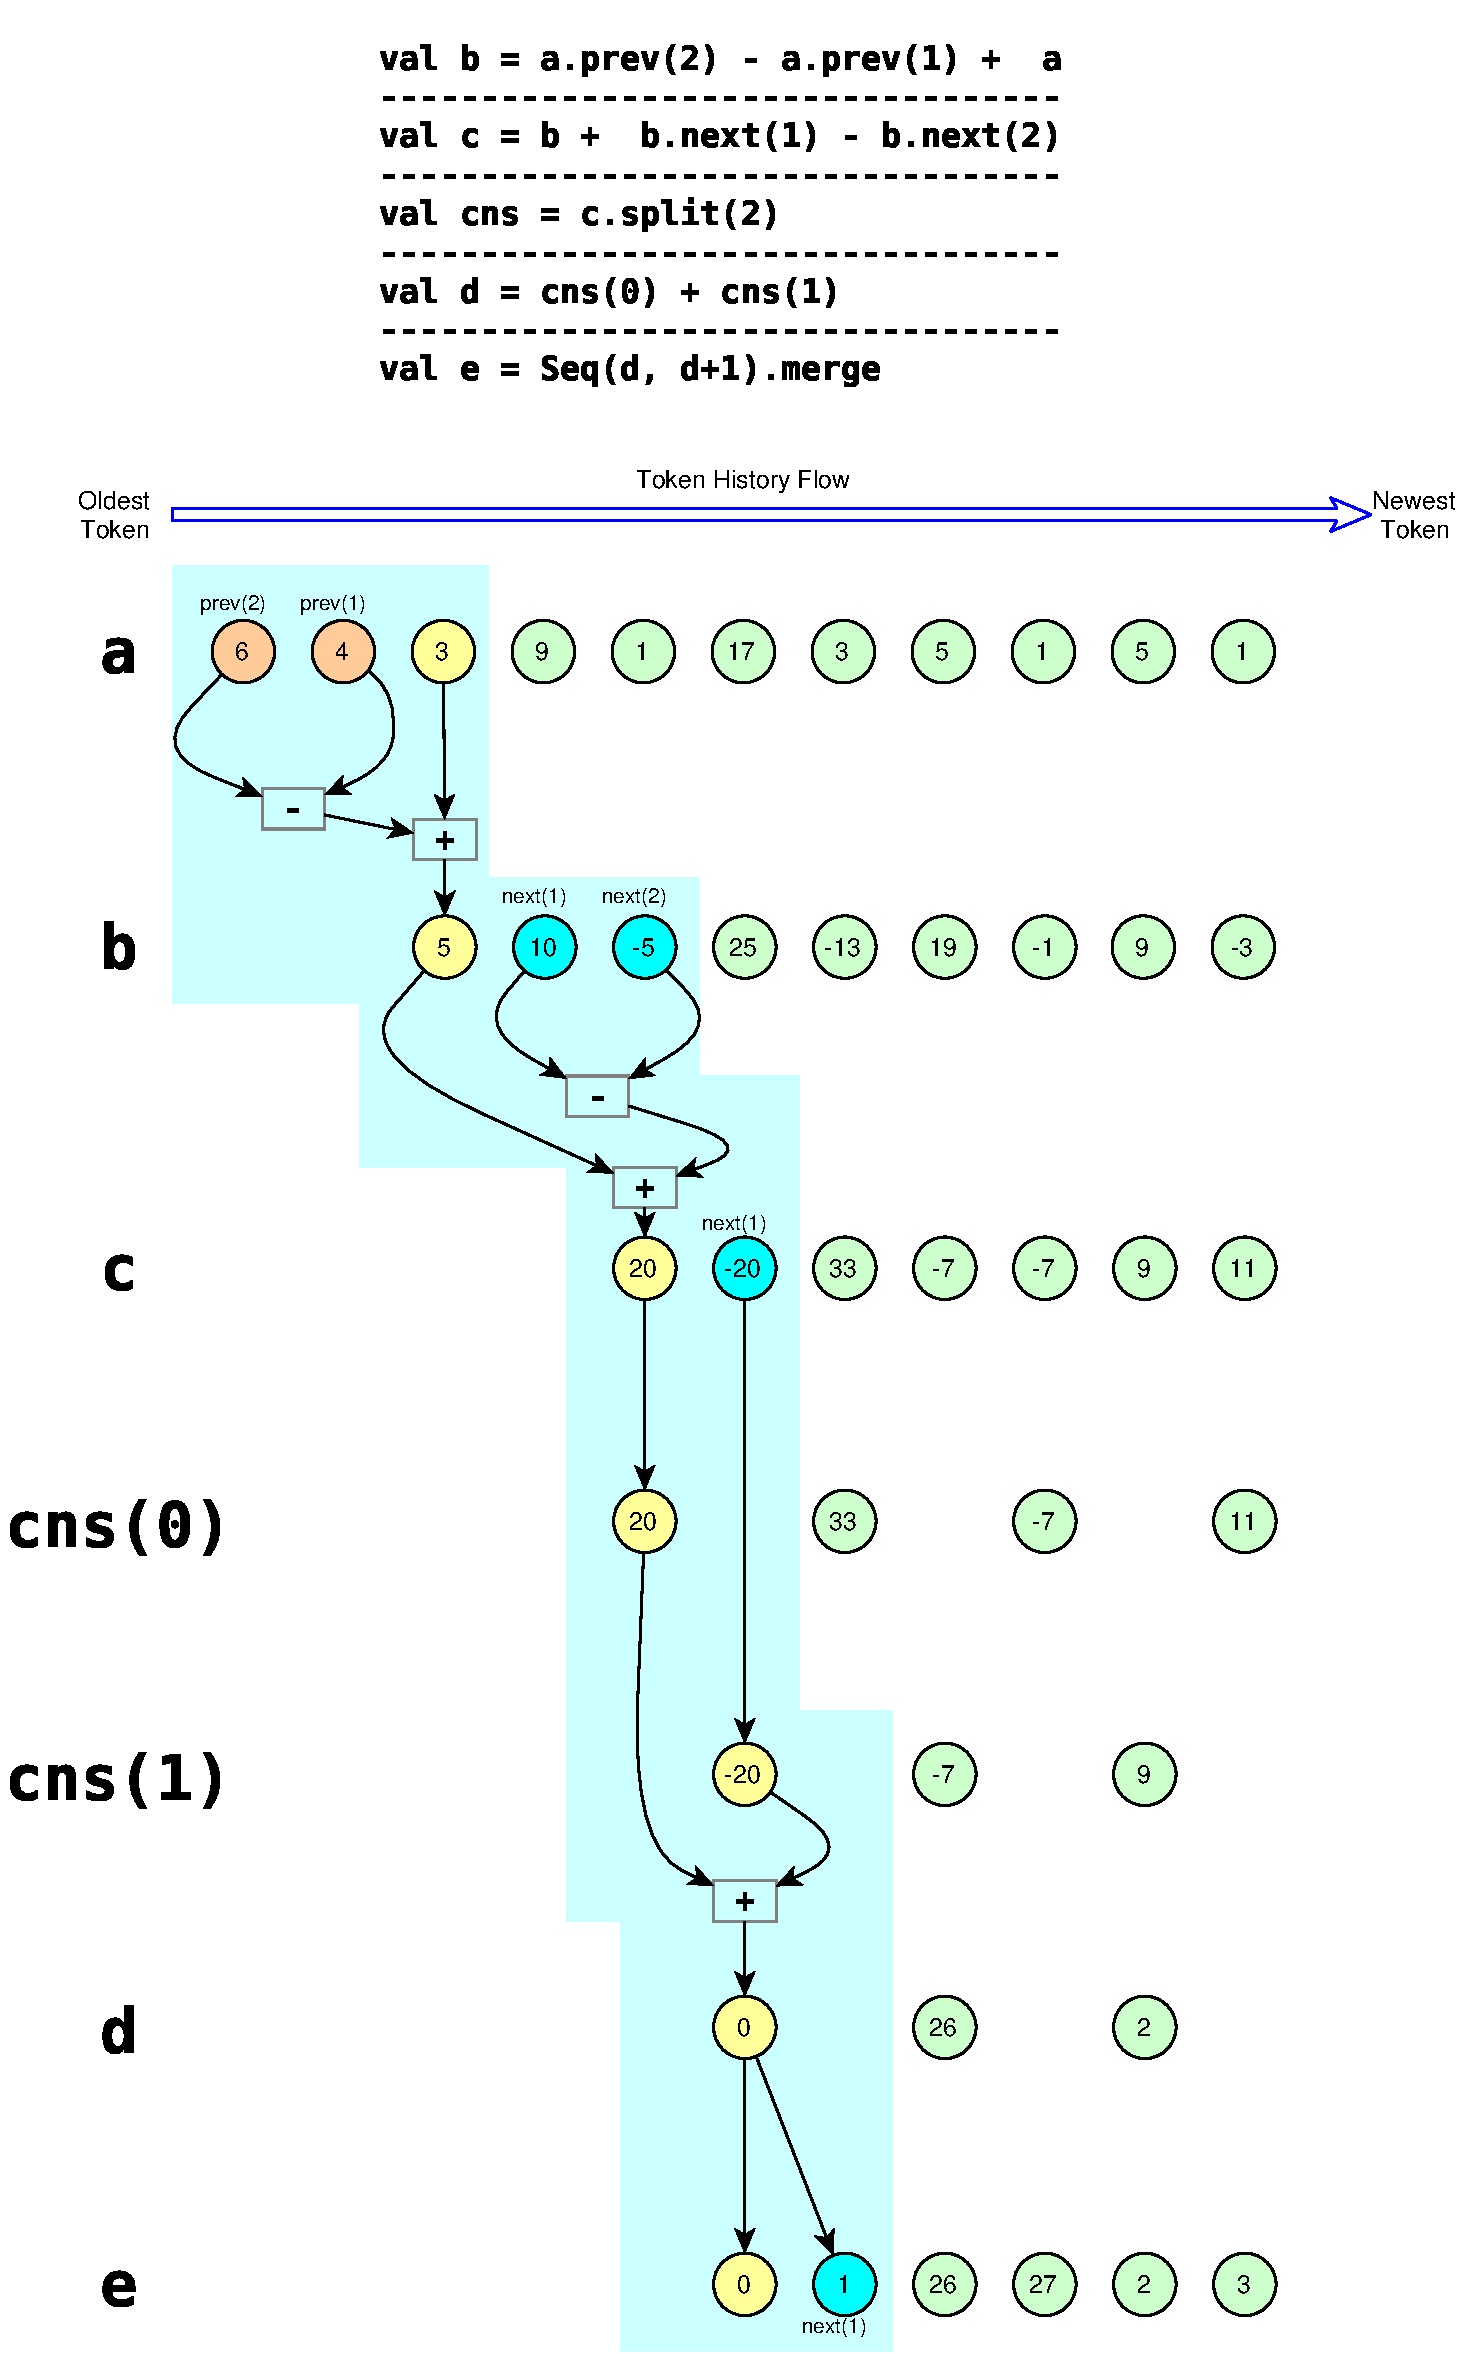
\includegraphics[width=\linewidth]{graphics/dataflow.pdf} 
  \captionof{figure}{Advanced static dataflow scheduling example}
  \label{fig:Dataflow}
\end{figure}

  
\section{Dynamic Dataflow Scheduling}
All static dataflow scheduling is \textit{blocking} and assumes a known fixed token rate. Allowing DFiant to handle dynamic dataflow scheduling, requires additional constructs to explicitly control the asynchronous FIFO-esque traits of its dataflow variables:
\begin{itemize}
  \item \code{.isNotEmpty}\quad This construct returns a boolean dataflow variable that is guaranteed to fire a single \code{true} token when the input receives a new token, but can fire an unbounded number of \code{false} tokens.
  \item \code{.dontConsume}\quad All dataflow variables are implicitly consumed in DFiant (unconnected outputs are semantically consumed as well, and are completely removed during compiler optimization). Multiple variables may consume from the same variable (dataflow fork), but if either requires to implement back-pressure, then \code{dontConsume} is used and all forked paths are delayed.
  \item \code{.isNotFull}\quad This construct returns a boolean dataflow variable that is guaranteed to fire a single \code{true} token when the output releases an old token, but can fire an unbounded number of \code{false} tokens.
  \item \code{.dontProduce}\quad All dataflow variables are implicitly produced in DFiant (to their previous value). Invoking \code{dontProduce} prevents value production. 

  \begin{figure}[H]
    \centering
    \begin{minipage}{0.49\linewidth}
      \begin{minted}[linenos,autogobble,tabsize=2,framesep=1pt, frame=single,fontsize=\scriptsize]{scala}
        def blockingMergeTwo[N](in0 : DFBits[N],
            in1 : DFBits[N]) : DFBits[N] = {
          val out = DFBits[N]
          val sel = DFBool := 0
        
          ifdf (!sel) {
            out := in0
            in1.dontConsume()
          } elsedf {
            out := in1
            in0.dontConsume()
          }
          
          
          
          
          sel := !sel
          out
        }
      \end{minted}
    \subcaption{Blocking round-robin merge example}
    \label{fig:BlockingRR}
   \end{minipage}%
   \hfill
   \begin{minipage}{0.49\linewidth}
      \begin{minted}[autogobble,tabsize=2,framesep=1pt, frame=single,fontsize=\scriptsize]{scala}
      def greedyMergeTwo[N](in0 : DFBits[N], 
          in1 : DFBits[N]) : DFBits[N] = {
        val out = DFBits[N]
        val sel = DFBool := 0
        
        ifdf (!sel && in0.isNotEmpty()) {
          out := in0
          in1.dontConsume()
        } elseifdf (sel && in1.isNotEmpty()) {
          out := in1
          in0.dontConsume()
        } elsedf {
          out.dontProduce()
          in0.dontConsume()
          in1.dontConsume()
        }
        sel := !sel
        out
      }
      \end{minted}
      \subcaption{Greedy round-robin merge example}
      \label{fig:GreedyRR}
    \end{minipage}
    \captionof{figure}{Blocking vs. Gready round-robin merge example}
    \label{fig:RRMerge}
  \end{figure}
\end{itemize}

\fig{fig:RRMerge} gives two possible round-robin \code{merge} implementations, using the dynamic control constructors. The blocking \code{merge} stops producing if either input stops producing, while the greedy \code{merge} can continue on toggling between inputs in search for new tokens to ouput.


